\documentclass[12pt]{amsart}

\usepackage{a4wide, amsxtra}

\usepackage[pdftex]{graphicx}

 \title{PMTH212 Assignment 7}

 \author{Mark Villar}

\begin{document} 

\maketitle 

\begin{enumerate}
	
	\item $f(x,y)=x^2+xy-2y-2x+1$
		\begin{align*}
			&f_x(x,y)=2x+y-2=0 \ \Rightarrow \ y=2-2x \\
			&f_y(x,y)=x-2=0 \ \Rightarrow \ x=2
		\end{align*}
		We obtain only one solution when $x=2, \ y=-2$. Hence there is a critical point  at $(2,-2)$.
		\begin{align*}
			&f_{xx}(x,y)=0, \ \ f_{yy}(x,y)=0, \ \ f_{xy}(x,y)=1 \\
			&D=f_{xx}f_{yy}-f^2_{xy}=2(0)-1^2=-1
		\end{align*}
		Since $D<0$ \ at $(2,-2)$, this critical point is a saddle point.
		
		\medskip
		
	\item $f(x,y)=xy-2x$ \ on the triangular region $R$ with vertices $(0,0), (0,4), (4,0)$
		\begin{align*}
			&f_x=y-2=0 \ \Rightarrow y=2 \\
			&f_y=x=0 \ \Rightarrow x=0
		\end{align*} 
		We obtain only one solution when $x=0, \ y=2$, with $f(0,2)=0$. Hence there is a critical point at $(0,2)$. A sketch of the region $R$ divided into three line segments $L_1, L_2, L_3$, reveals $(0,2)$ is a boundary point of $R$, lying on $L_1$. \\
		\begin{figure}[h]
			\centering
			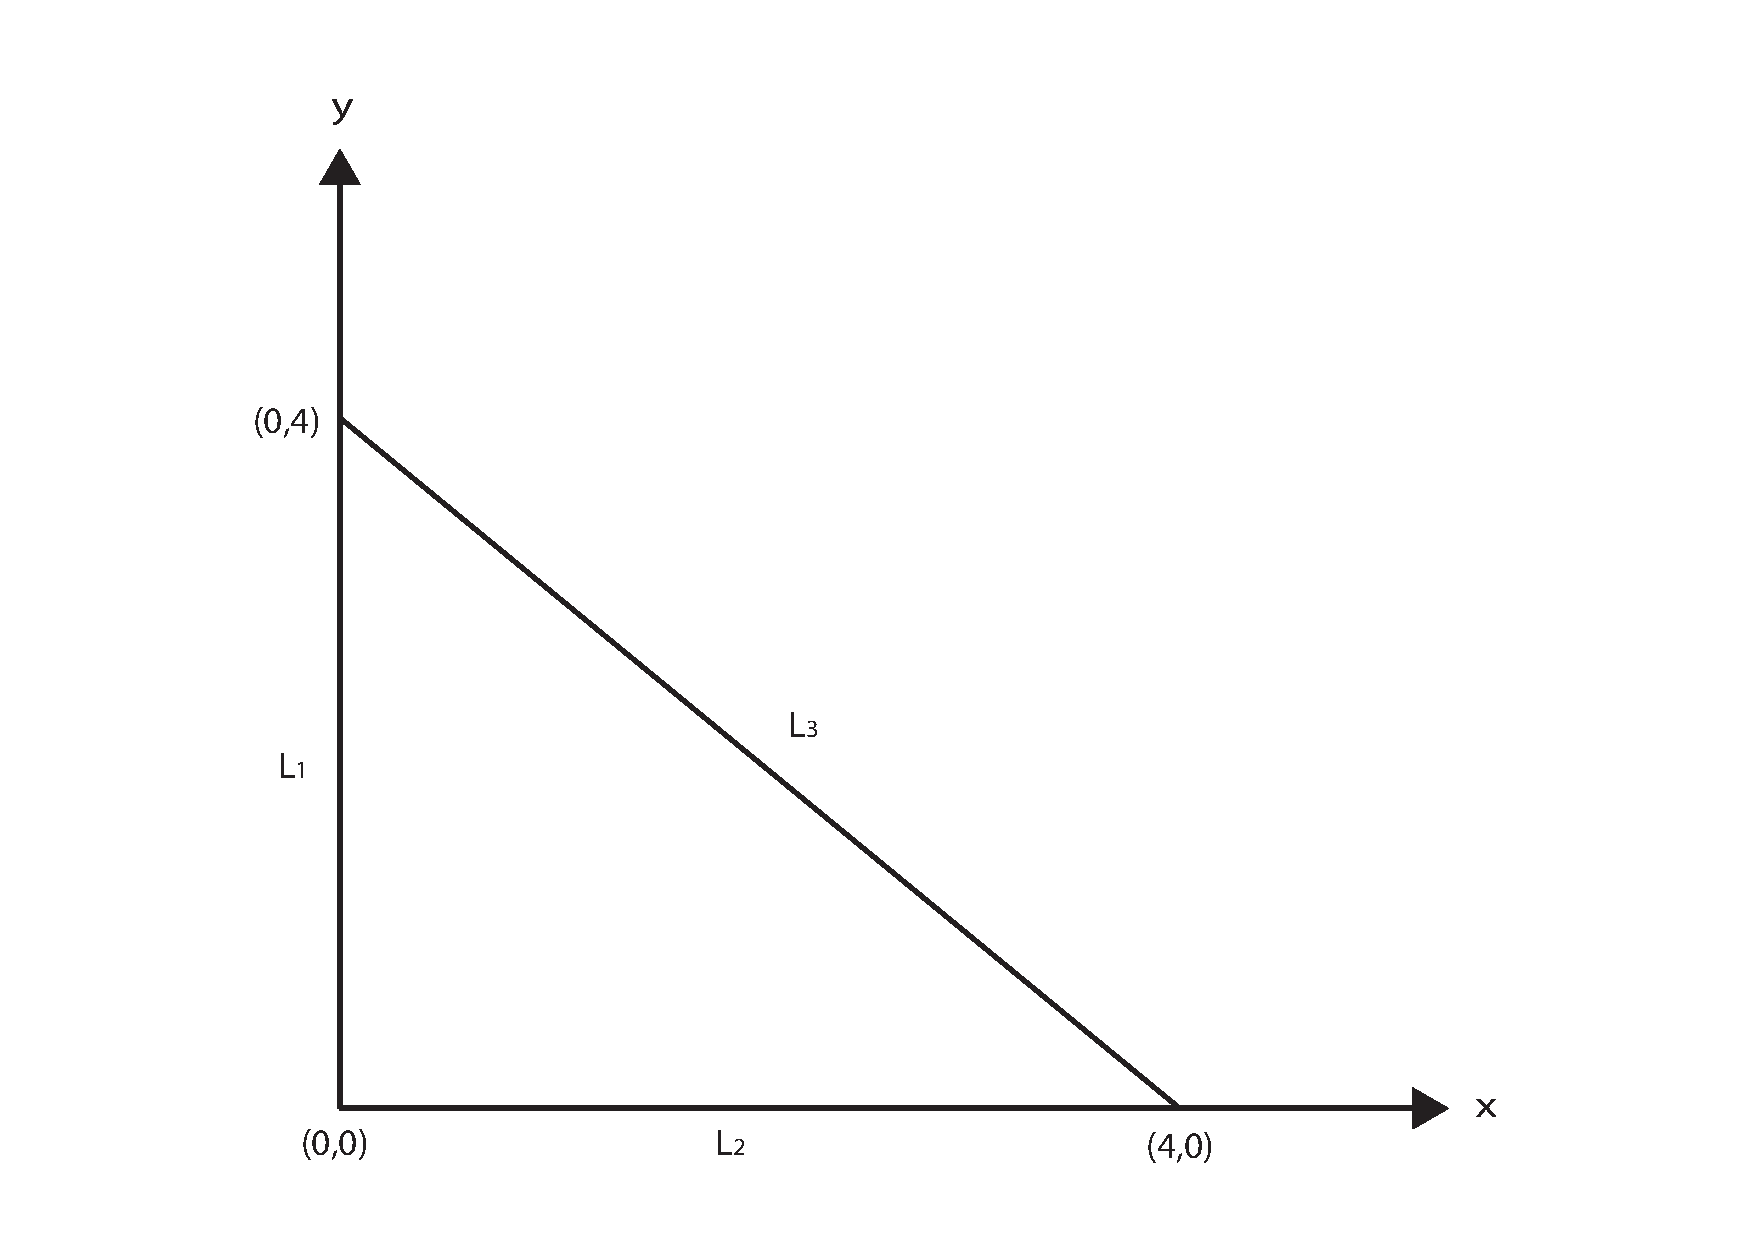
\includegraphics[width=4.4in]{Boundary.pdf}
		\end{figure}
		\\
		$L_1$: $x=0$ \ and \ $f(x,y)=f(0,y)=0$, \ $0\le y \le 4$ \ \text{(monotone)}\\
		$L_2$: $y=0$ \ and \ $f(x,y)=f(x,0)=-2x$, \ $0\le x \le 4$ \ \text{(monotone)} \\
		$L_3$: $y=4-x$ \ and \ $f(x,y)=f(x,4-x)=2x-x^2$, \ $0\le x \le 4$ \\
		\\
		On $L_1$, $f$ has no critical points and the value of $f$ is 0, regardless of $y$. In fact, $f$ is simply the $y$-axis on the closed interval $[0,4]$. Hence, the minimum and maximum are both 0, attained along the entire boundary line. \\
		\\
		On $L_2$, $f$ has no critical points and the maximum is clearly 0 attained at $(0,0)$ while the minimum is $-8$ attained at $(4,0)$. \\
		\\
		On $L_3$, $g(x)=2x-x^2$, \ $g'(x)=2-2x=0 \ \Rightarrow \ x=1, \ y=3$, \ $g''(x)<0$, \ $f(1,3)=1$. Hence, we obtain a maximum of $1$  at $(1,3)$. \\
	 \\
	 Combining results from the three line segements, we find the maximum on the boundary is $1$ and the minimum is $-8$. \\
	 \\
	 Therefore the absolute maximum of $f$ over $R$ is $1$ attained at $(1,3)$ while the absolute minimum is $-8$ attained at $(4,0)$.\\

	\item $f(x,y)=x^2-y$, \ \ $ g(x,y)=x^2+y^2-25=0$, \ \ $\nabla f(x,y)= \lambda \nabla g(x,y)$
		\begin{align*}
			\ &\nabla f(x,y)=2x\vec{i}-\vec{j} &\nabla g(x,y)=2x\vec{i}+2y\vec{j}\\
			&2x=\lambda 2x \ \Rightarrow \lambda=1,  \ x\ne0 &-1=\lambda 2y \ \Rightarrow \ y=-\frac{1}{2} \\
			&x^2+\left(-\frac{1}{2}\right)^2=25 &x^2=\frac{99}{4} \ \Rightarrow \ x=\pm \frac{3\sqrt{11}}{2}
		\end{align*}
		Hence $\left(-\dfrac{3\sqrt{11}}{2},-\dfrac{1}{2}\right)$ and $\left(\dfrac{3\sqrt{11}}{2},-\dfrac{1}{2}\right)$ are critical points when $x\ne0$. \\
		\\
		When $x=0$, we compute $y$ from the constraint and obtain the corresponding $\lambda$-values as follows.
			\begin{align*}
				&y=\pm\sqrt{25-x^2}=\pm\sqrt{25-0^2}=\pm 5 \\
				&-1=\lambda 2y=\lambda 2(5) \ \Rightarrow \ \lambda=-\frac{1}{10} \\
				&-1=\lambda 2y=\lambda 2(-5) \ \Rightarrow \ \lambda=\frac{1}{10}
			\end{align*}
		Substituting the $\lambda$-values back into $y=-\dfrac{1}{2\lambda}$, we obtain two more critical points at $(0,-5)$ and $(0,5)$. \\
		\begin{table}[!ht]
			\begin{center}
				\begin{tabular}{|c||c|c|c|c|}
					\hline
					$(x,y)$ &$(0,-5)$ &$(0,5)$ &$(-\frac{3\sqrt{11}}{2},-\frac{1}{2})$ &$(\frac{3\sqrt{11}}{2},-\frac{1}{2})$ \\
					\hline
					$f(x,y)$ &5 &$-5$ &$25 \frac{1}{4}$ &$25 \frac{1}{4}$ \\
					\hline
				\end{tabular}
			\end{center}
		\end{table} 
		\\
		We conclude from the table above that the maximum is \ $25 \dfrac{1}{4}$ attained at $\left(\pm\dfrac{3\sqrt{11}}{2},-\dfrac{1}{2}\right)$ while the minimum is $-5$ attained at $(0,5)$.\\
		
		\medskip
		
	\item $D(x,y)=x^2+y^2, \ \ g(x,y)=2x-4y-3=0, \ \ \nabla D(x,y)=\lambda \nabla g(x,y)$
	\begin{align*}
		\ \ \ \ &\nabla D(x,y)=2x\vec{i}+2y\vec{j} &\nabla g(x,y)=2\vec{i}-4\vec{j}\\
		&2x=2\lambda \ \Rightarrow x=\lambda &2y=-4\lambda \ \Rightarrow \ y=-2\lambda=-2x \\
		&2x-4(-2x)-3=0 \ \Rightarrow 10x-3=0 &x=\frac{3}{10}, \ y=-2\left(\frac{3}{10}\right)=-\frac{3}{5} \\
	&d(x,y)=\sqrt{x^2+y^2} &d\left(\frac{3}{10},-\frac{3}{5}\right)=\sqrt{\frac{9}{100}+\frac{36}{100}}=\frac{3\sqrt{5}}{10}
	\end{align*}
	We use the second derivative test to confirm that the critical point is a minimum.
	\begin{align*}
		&D_x=2x, \ \ D_y=2y, \ \ D_{xx}=2, \ \ D_{yy}=2, \ \ D_{xy}=0 \\
		&T=D_{xx}D_{yy}-D^2_{xy}=2(2)-0^2=4>0
	\end{align*}
	Since $D_{xx}>0$ and $T>0$, the critical point is a minimum. Hence the point on the line closest to the origin is $\left(\dfrac{3}{10},-\dfrac{3}{5}\right)$ with a distance of $\dfrac{3\sqrt{5}}{10}$.
					
\end{enumerate}

\end{document}
